\section{如何识别GPU架构与代际}

\subsection{使用TechPowerUp查询规格}

下面我们以 RTX 3090 和 A100 GPU 为例，介绍如何快速获取这些规格参数。

方法很简单：推荐使用 TechPowerUp 网站（\href{https://www.techpowerup.com/gpu-specs/a100-pcie-80-gb.c3821}{A100 页面}），
它收录了各大厂商详尽的 GPU 数据库。你只需在搜索引擎中输入"A100 GPU TechPowerUp"并回车，点击搜索结果中的对应链接，
即可查看该显卡的完整规格与详细信息。

\begin{figure}
    \centering
    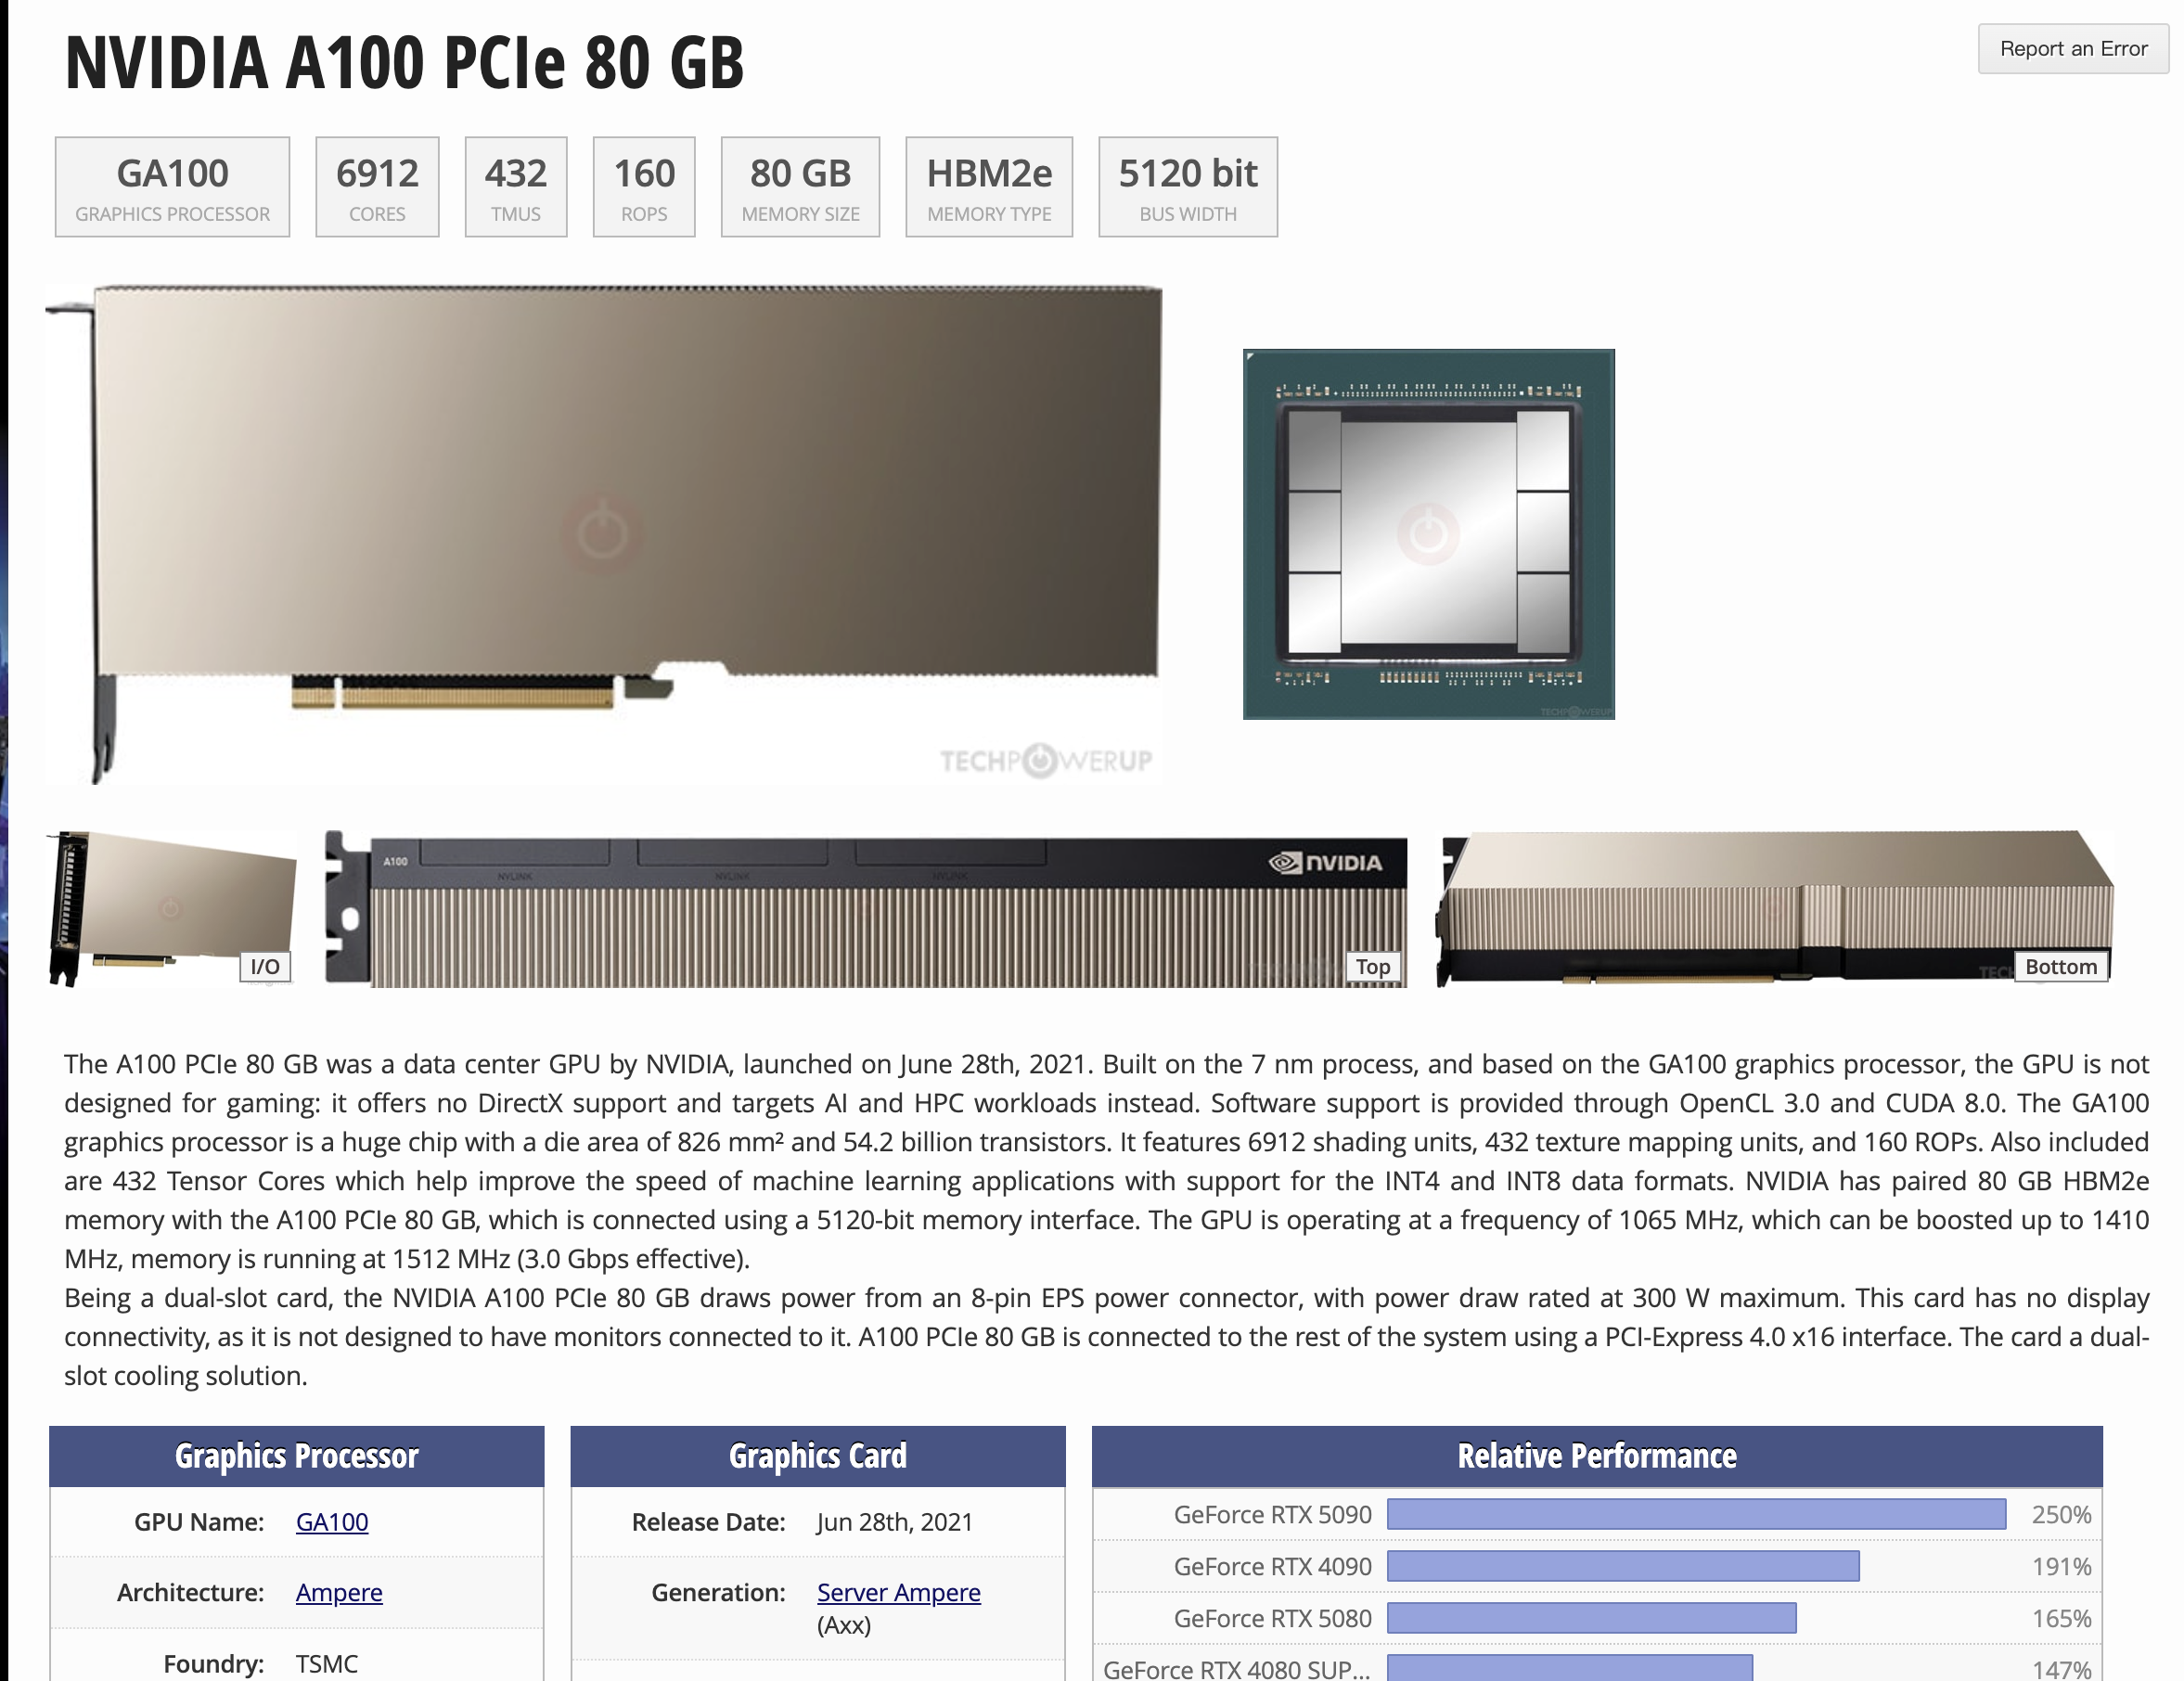
\includegraphics[width=0.75\linewidth]{resources/cuda-015.png}
    \caption{A100 GPU架构}
    \label{fig:placeholder}
\end{figure}

同样，你可以在 TechPowerUp（\href{https://www.techpowerup.com/gpu-specs/geforce-rtx-3090.c3622}{RTX 3090 页面}）
查 RTX 3090 的规格。现在对这两款 GPU 做一个简单的比较：首先是 GPU 芯片代号——A100 的代号为 GA100。关于 GPU 芯
片的具体含义我们将在后续章节中解释，这里只需关注它的名称。然后看核心数量：A100 拥有约 7000 个核心，而 RTX 3090 拥有
超过一万个核心。

\begin{figure}
    \centering
    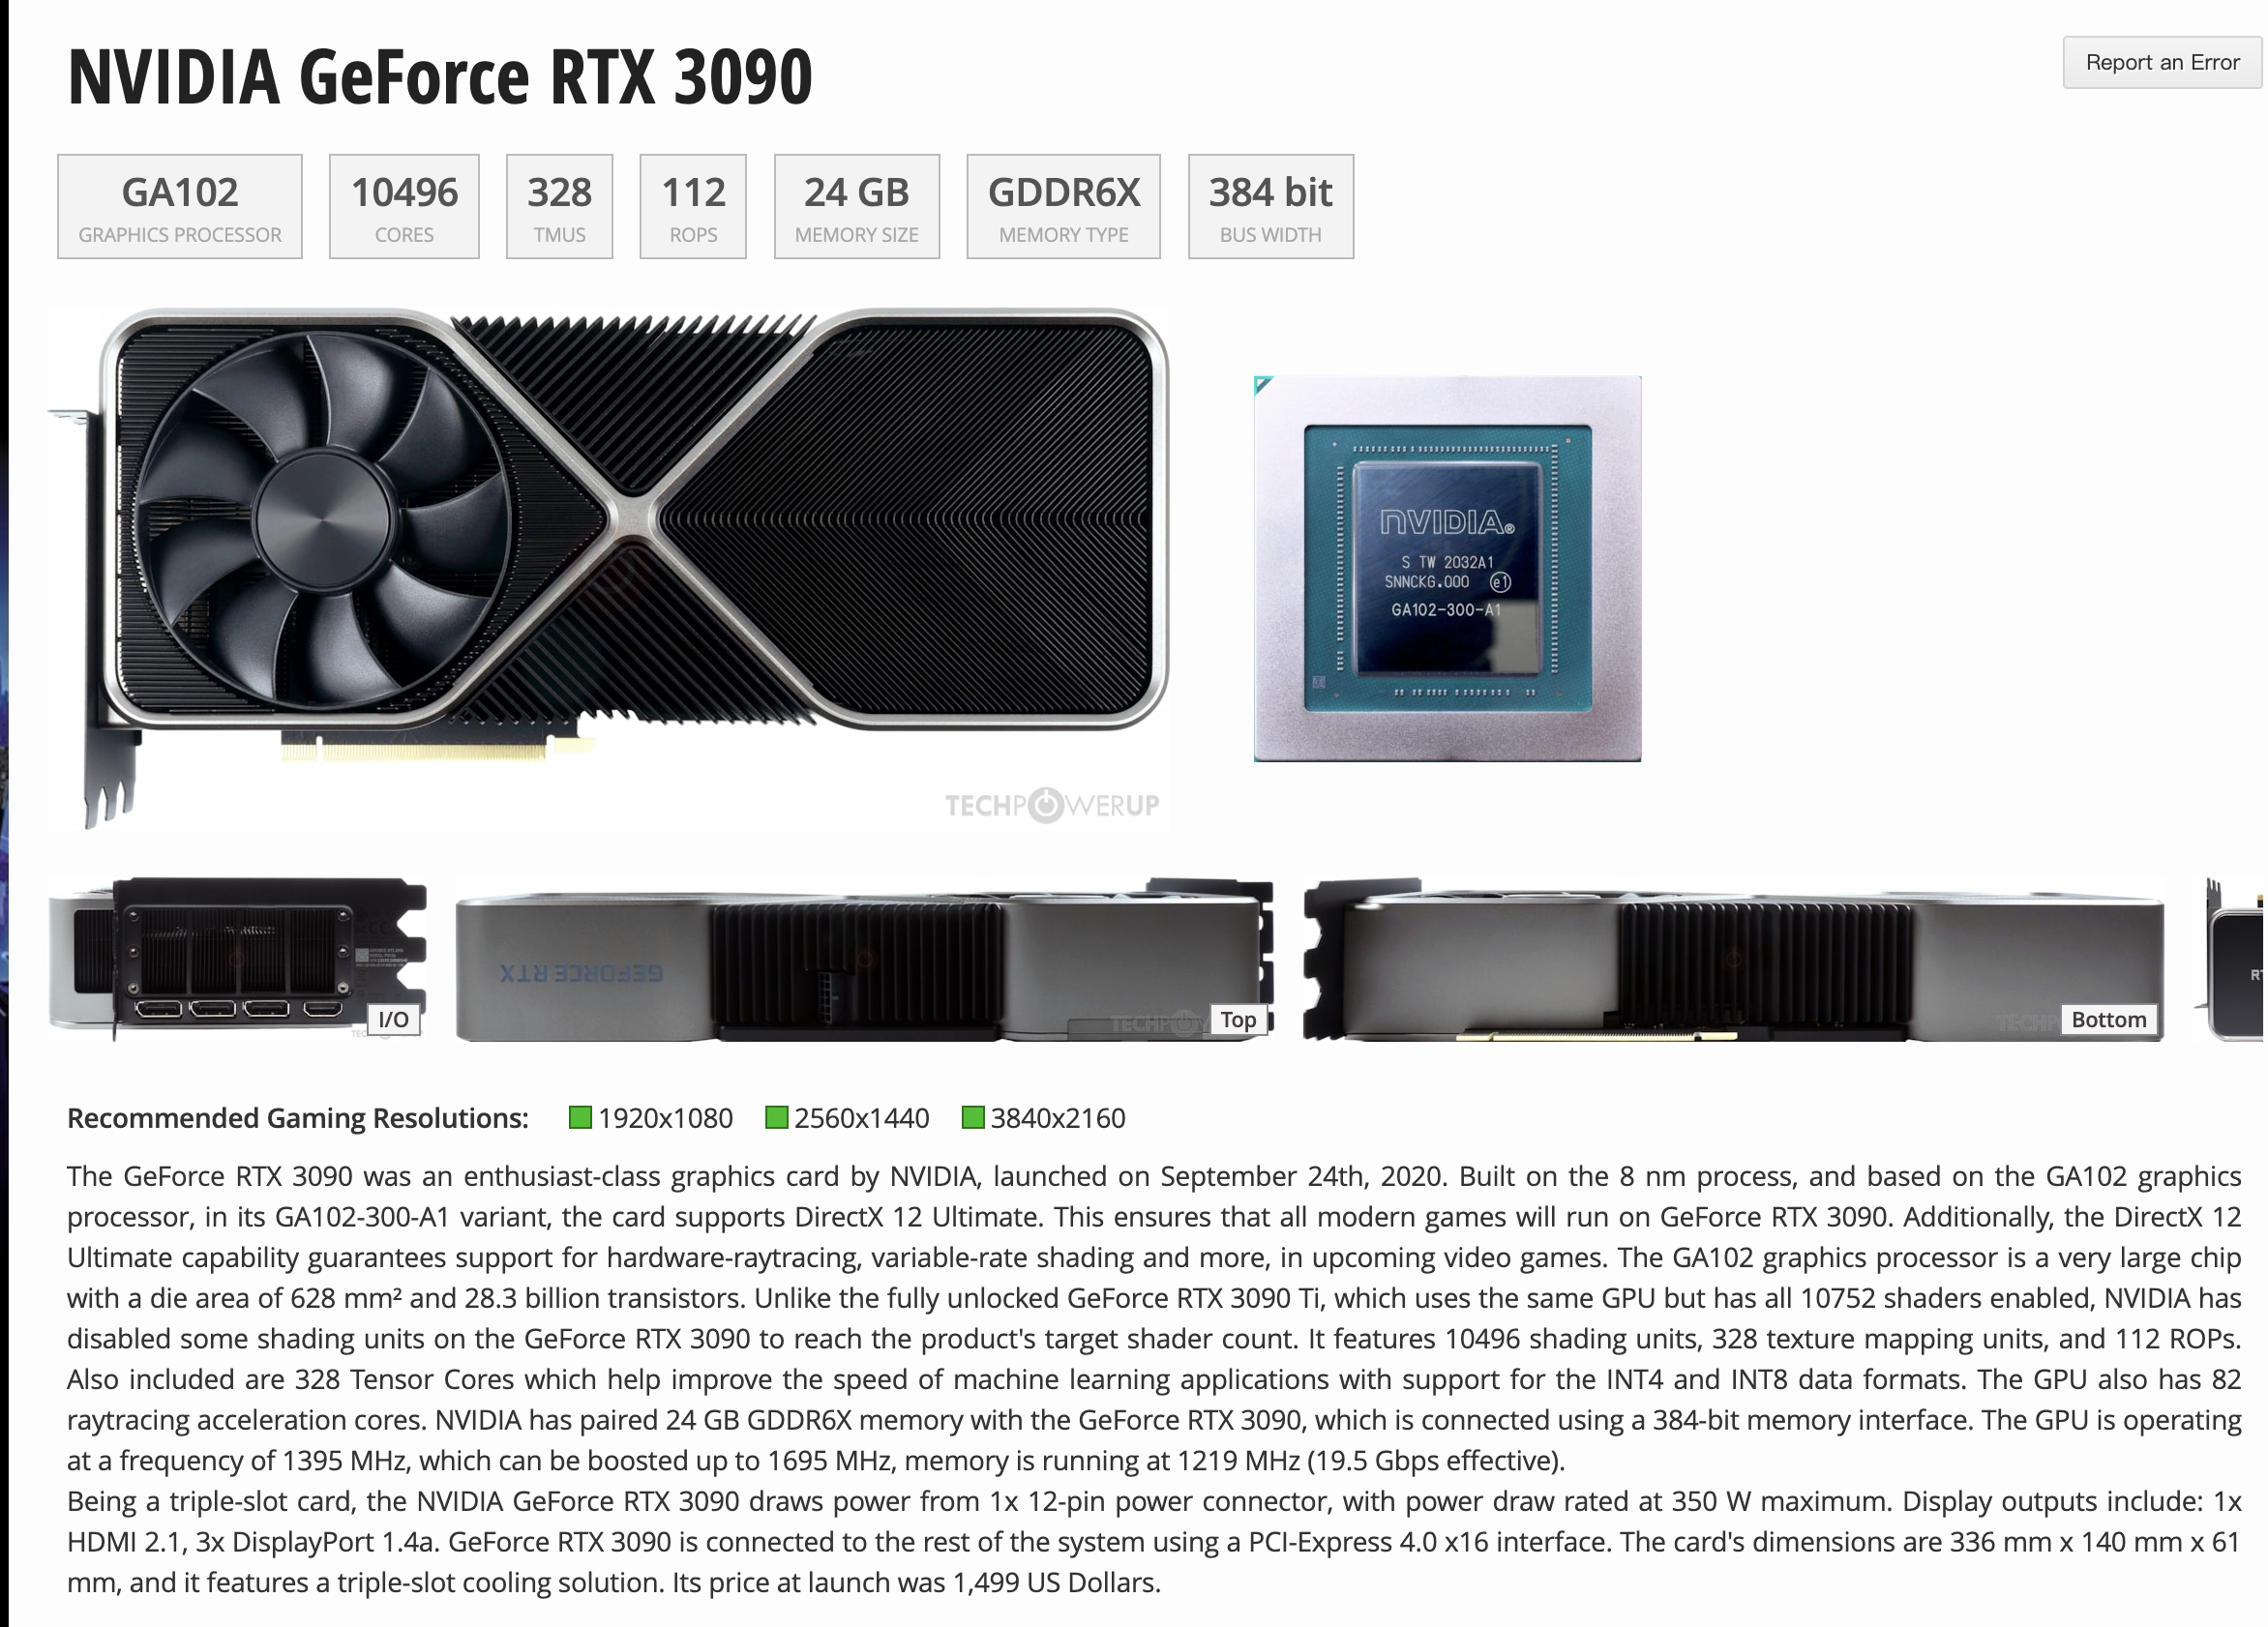
\includegraphics[width=0.75\linewidth]{resources/cuda-016.png}
    \caption{RTX 3090 GPU架构}
    \label{fig:placeholder}
\end{figure}

你在这里也可以看到许多规格参数，解释了每款 GPU 的不同能力。但本文先跳过这些，只关注世代和架构，后续章节将详细讨论更多
规格。不过请记住 6192 这个数字——这是专用于处理单精度运算的核心数量，并不代表用于各种操作的总核心数。举例来说，A100 
GPU 还包含用于处理整数运算和双精度运算的核心。这些将在后续章节中从官方白皮书和数据表中深入探讨，本文暂不展开。

\subsection{A100与RTX 3090架构对比}

现在让我们聚焦于这些 GPU 的世代和架构。以 RTX 3090 为例，其世代为 GeForce 30，架构为 Ampere。你还记得 GeForce 是
为谁设计的吗？正如上一章所述，它是为普通台式机、笔记本电脑和工作站设计的。

再来看 A100 GPU，其世代是 Tesla，正如前文所述，Tesla 世代专用于 HPC 服务器和超级计算机。值得关注的是，A100 与 RTX 
3090 共享相同的 Ampere 架构，尽管它们是为不同的应用场景而设计的。

这里引出一个重要问题：我们如何从外观上确认 GeForce 与 Tesla 世代之间的区别？


\subsection{视觉区分GeForce与Tesla}

检查这些 GPU 的图片时，你会注意到 Tesla GPU 通常没有板载冷却风扇。如果你看 A100 GPU 的图片，找不到任何冷却风扇。同样
，V100 GPU 也属于 Tesla 世代，搜索它的图片，可以看到它也不包含冷却风扇。其原因是这些 GPU 设计用于 HPC 环境，而这些环
境中配备了外部且更强大的冷却系统——如果你搜索全球任何超级计算中心的照片，就能看到其冷却系统的复杂性。

另一方面，GeForce GPU（例如我们电脑中的 RTX 系列）通常都配备内置风扇。这些风扇是标准台式机或工作站环境中散热所必需的
。这就是我们从外观上确认 GeForce 和 Tesla 世代之间区别的方法：Tesla GPU 无冷却风扇，GeForce GPU 有冷却风扇——原因就
在于它们所使用的目标环境不同。

